\documentclass[12pt]{scrartcl}

\input{../styles/Packages}
\input{../styles/FormatAndHeader}

% Zusätzliche Pakete für das Use-Case-Diagramm (TikZ)
\usepackage{tikz}
\usetikzlibrary{arrows.meta, calc, shapes.geometric}
\usepackage{enumitem}
\usepackage{pdflscape}

% Hilfsbefehl für UML-Stereotypen
\newcommand{\umark}[1]{\guillemotleft #1\guillemotright}

\setcounter{sheetnr}{8}   % Übungsblatt 8
\setcounter{exnum}{1}     % Aufgabe 1

\begin{document}

% ==============================================================
%  Aufgabe 8.1: UML Use-Case-Diagramm
% ==============================================================
    \exercise{Abgabe 8.1: UML Use-Case-Diagramm}

% --------------------------------------------------------------
%  Use-Case-Diagramm
% --------------------------------------------------------------
    \subsection*{Use-Case-Diagramm}

    \begin{figure}[htbp]
        \centering
        \resizebox{\textwidth}{!}{%
            \begin{tikzpicture}[
            % ----- Styles -----
                uc/.style={
                    ellipse, draw=black, thick,
                    minimum width=3.2cm, minimum height=1.3cm,
                    text centered, font=\footnotesize, align=center
                },
                rel/.style={-{Stealth[length=2.5mm]}, dashed, thick},
                assoc/.style={thick},
                lbl/.style={font=\scriptsize, fill=white, inner sep=1pt}
            ]

% ===================== Systemgrenze ============================
% Breiter Rahmen: linke Spalte (x=0) + rechte Spalte (x=6)
                \draw[thick, rounded corners=6pt] (-5.5, 1.5) rectangle (10, -17.5);
                \node[font=\large\bfseries] at (2.25, 1) {Online-Banking System};

% ===================== Use Cases (Ovale) =======================
%
%  Layout: zwei Spalten, damit Include-Pfeile zu "Anmelden"
%  durch die Lücke zwischen den Spalten verlaufen.
%
%  Linke Spalte (x=0):   Kontostand, Umsätze, Überweisung
%  Rechte Spalte (x=6):  Anmelden, Kto drucken, Auszug drucken
%  Untere Reihe:          Daten, TAN, Geldtransfer, Kto sperren, MA info

                \node[uc] (uc1)  at (6,     0)      {Anmelden};

                \node[uc] (uc2)  at (0,    -3)      {Kontostand\\anzeigen};
                \node[uc] (uc3)  at (6,    -3)      {Kontostand\\drucken};

                \node[uc] (uc4)  at (0,    -6)      {Ums\"atze\\anzeigen};
                \node[uc] (uc5)  at (6,    -6)      {Kontoauszug\\drucken};

                \node[uc] (uc6)  at (0,    -9)      {\"Uberweisung\\t\"atigen};

                \node[uc] (uc7)  at (-3,   -12.5)   {Daten\\eingeben};
                \node[uc] (uc8)  at (3,    -12.5)   {TAN\\abfragen};
                \node[uc] (uc9)  at (-3,   -15.5)   {Geldtransfer\\durchf\"uhren};
                \node[uc] (uc10) at (7.5,  -12.5)   {Konto\\sperren};
                \node[uc] (uc11) at (7.5,  -15.5)   {Mitarbeiter\\informieren};

% ===================== Akteur: Bankkunde =======================
                \draw (-7.5, -4.7)  circle (0.35);
                \draw (-7.5, -5.05) -- (-7.5, -6.0);
                \draw (-8, -5.5) -- (-7.5, -5.3) -- (-7, -5.5);
                \draw (-7.5, -6.0)  -- (-7.85, -6.8);
                \draw (-7.5, -6.0)  -- (-7.15, -6.8);
                \node[below, font=\bfseries\small] at (-7.5, -6.9) {Bankkunde};

% ===================== Akteur: Mitarbeiter =====================
                \draw (12, -14.2) circle (0.35);
                \draw (12, -14.55) -- (12, -15.5);
                \draw (11.5, -15.0) -- (12, -14.8) -- (12.5, -15.0);
                \draw (12, -15.5) -- (11.65, -16.3);
                \draw (12, -15.5) -- (12.35, -16.3);
                \node[below, font=\bfseries\small] at (12, -16.4) {Mitarbeiter};

% ===================== Assoziationen ===========================
                \draw[assoc] (-7, -5.3) -- (uc2.west);
                \draw[assoc] (-7, -5.6) -- (uc4.west);
                \draw[assoc] (-7, -5.8) -- (uc6.west);
                \draw[assoc] (uc11.east) -- (11.5, -15.0);

% ===================== <<include>>-Beziehungen =================
%
% Hauptanwendungsfälle → Anmelden
% Die Pfeile verlaufen diagonal durch die Lücke
% zwischen linker und rechter Spalte -- keine Überlappung!
%
                \draw[rel] (uc2) -- (uc1)
                node[lbl, pos=0.5, above] {\umark{include}};
                \draw[rel] (uc4) -- (uc1)
                node[lbl, pos=0.35, above left] {\umark{include}};
                \draw[rel] (uc6) -- (uc1)
                node[lbl, pos=0.25, left] {\umark{include}};

% Überweisung → Teilschritte
                \draw[rel] (uc6) -- (uc7)
                node[lbl, midway, left] {\umark{include}};
                \draw[rel] (uc6) -- (uc8)
                node[lbl, midway, right] {\umark{include}};
                \draw[rel] (uc6) -- (uc9)
                node[lbl, pos=0.5, left] {\umark{include}};

% Konto sperren → Mitarbeiter informieren
                \draw[rel] (uc10) -- (uc11)
                node[lbl, midway, right] {\umark{include}};

% ===================== <<extend>>-Beziehungen ==================
                \draw[rel] (uc3) -- (uc2)
                node[lbl, midway, above] {\umark{extend}};
                \draw[rel] (uc5) -- (uc4)
                node[lbl, midway, above] {\umark{extend}};

% Konto sperren → TAN abfragen
                \draw[rel] (uc10) -- (uc8)
                node[lbl, midway, above] {\umark{extend}};
                \node[font=\scriptsize, text width=2.8cm, align=center]
                at (5.25, -13.3) {[Bedingung:\\3$\times$ falsche TAN]};

            \end{tikzpicture}
        }% end resizebox
        \caption{UML Use-Case-Diagramm -- Online-Banking System}
        \label{fig:usecase}
    \end{figure}

    \newpage

% ==============================================================
%  Textuelle Beschreibung der Use Cases
% ==============================================================
    \subsection*{Textuelle Beschreibung der Use Cases}

% ---------------------------------------------------------------
    \paragraph{UC1 -- Anmelden}~\\[4pt]
    \begin{description}[leftmargin=4.5cm, style=nextline, font=\normalfont\bfseries]
  \item[Name und Kurzbeschreibung:]
  \textbf{Anmelden.}
  Der Bankkunde meldet sich mit seinen Zugangsdaten (Kontonummer und PIN) beim
  Online-Banking-System an, um auf die verf\"ugbaren Funktionen zugreifen zu k\"onnen.

  \item[Vorbedingung:]
  Das Online-Banking-System ist erreichbar. Der Kunde besitzt g\"ultige Zugangsdaten.

  \item[Nachbedingung:]
  Der Kunde ist authentifiziert und hat Zugang zu allen Funktionen des Systems
  (Kontostand, Ums\"atze, \"Uberweisung).

  \item[Fehlersituationen:]
  Ung\"ultige Zugangsdaten (falsche Kontonummer oder falsche PIN).

  \item[Systemzustand im Fehlerfall:]
  Der Kunde ist nicht angemeldet. Das System verbleibt auf der Anmeldeseite
  im Status quo ante.

  \item[Akteure:]
  Bankkunde (prim\"arer Akteur).

  \item[Trigger:]
  Der Kunde ruft die Anmeldeseite des Online-Banking-Systems auf.

  \item[Standardablauf:]~
  \begin{enumerate}
      \item Der Kunde gibt seine Kontonummer und PIN ein.
      \item Das System pr\"uft die eingegebenen Zugangsdaten.
      \item Die Zugangsdaten sind korrekt; der Kunde wird zum Hauptmen\"u
      weitergeleitet.
  \end{enumerate}

  \item[Alternativablauf:]~
  \begin{itemize}
      \item[(2')] Die Zugangsdaten sind ung\"ultig. Das System zeigt eine
      Fehlermeldung an. Der Kunde wird aufgefordert, die Daten erneut
      einzugeben. Weiter mit Schritt~1.
  \end{itemize}
    \end{description}

% ---------------------------------------------------------------
    \paragraph{UC2 -- Kontostand anzeigen}~\\[4pt]
    \begin{description}[leftmargin=4.5cm, style=nextline, font=\normalfont\bfseries]
  \item[Name und Kurzbeschreibung:]
  \textbf{Kontostand anzeigen.}
  Der angemeldete Bankkunde l\"asst sich den aktuellen Kontostand seines Kontos
  auf dem Bildschirm anzeigen.

  \item[Vorbedingung:]
  Der Kunde ist erfolgreich angemeldet (\umark{include} Anmelden, UC1).

  \item[Nachbedingung:]
  Der aktuelle Kontostand wird dem Kunden auf dem Bildschirm dargestellt.

  \item[Fehlersituationen:]
  Kontodaten k\"onnen nicht abgerufen werden (z.\,B.\ interner Systemfehler).

  \item[Systemzustand im Fehlerfall:]
  Fehlermeldung wird angezeigt. Keine \"Anderung am System; der Kunde
  verbleibt im Hauptmen\"u.

  \item[Akteure:]
  Bankkunde (prim\"arer Akteur).

  \item[Trigger:]
  Der Kunde w\"ahlt die Funktion \glqq Kontostand anzeigen\grqq{} im Hauptmen\"u.

  \item[Standardablauf:]~
  \begin{enumerate}
      \item \umark{include} Anmelden (UC1).
      \item Der Kunde w\"ahlt die Funktion \glqq Kontostand anzeigen\grqq.
      \item Das System ruft den aktuellen Kontostand des Kunden ab.
      \item Der Kontostand wird dem Kunden angezeigt.
  \end{enumerate}

  \item[Alternativablauf:]~
  \begin{itemize}
      \item[(4')] Der Kunde w\"ahlt optional die Funktion \glqq Drucken\grqq.\\
      \umark{extend} Kontostand drucken (UC3).
  \end{itemize}
    \end{description}

% ---------------------------------------------------------------
    \paragraph{UC3 -- Kontostand drucken}~\\[4pt]
    \begin{description}[leftmargin=4.5cm, style=nextline, font=\normalfont\bfseries]
  \item[Name und Kurzbeschreibung:]
  \textbf{Kontostand drucken.}
  Der Kunde kann den aktuell angezeigten Kontostand auf Wunsch ausdrucken.
  Dieser Use Case erweitert UC2 (Kontostand anzeigen).

  \item[Vorbedingung:]
  Der Kontostand wird dem Kunden gerade angezeigt (UC2 ist aktiv).

  \item[Nachbedingung:]
  Ein Druckauftrag f\"ur den Kontostand wurde erfolgreich erzeugt und
  an den Drucker gesendet.

  \item[Fehlersituationen:]
  Drucker ist nicht verf\"ugbar oder Druckauftrag schl\"agt fehl.

  \item[Systemzustand im Fehlerfall:]
  Fehlermeldung wird angezeigt. Der Kontostand bleibt auf dem Bildschirm
  sichtbar; kein Druckauftrag wurde gesendet.

  \item[Akteure:]
  Bankkunde (prim\"arer Akteur).

  \item[Trigger:]
  Der Kunde w\"ahlt die Funktion \glqq Drucken\grqq{} innerhalb der
  Kontostandanzeige.

  \item[Standardablauf:]~
  \begin{enumerate}
      \item Der Kunde w\"ahlt \glqq Drucken\grqq.
      \item Das System erzeugt eine druckbare Ansicht des Kontostands.
      \item Der Druckauftrag wird an den Drucker gesendet.
      \item Der Kunde erh\"alt eine Best\"atigung \"uber den erfolgreichen Druck.
  \end{enumerate}

  \item[Alternativablauf:]
  --

  \item[Beziehung:]
  \umark{extend} UC2 -- Kontostand anzeigen.
    \end{description}

% ---------------------------------------------------------------
    \paragraph{UC4 -- Ums\"atze anzeigen}~\\[4pt]
    \begin{description}[leftmargin=4.5cm, style=nextline, font=\normalfont\bfseries]
  \item[Name und Kurzbeschreibung:]
  \textbf{Ums\"atze anzeigen.}
  Der angemeldete Bankkunde l\"asst sich die Kontoumsätze der letzten drei Monate
  auf dem Bildschirm anzeigen.

  \item[Vorbedingung:]
  Der Kunde ist erfolgreich angemeldet (\umark{include} Anmelden, UC1).

  \item[Nachbedingung:]
  Die Ums\"atze der letzten drei Monate werden dem Kunden auf dem
  Bildschirm dargestellt.

  \item[Fehlersituationen:]
  Umsatzdaten k\"onnen nicht abgerufen werden (z.\,B.\ interner Systemfehler).

  \item[Systemzustand im Fehlerfall:]
  Fehlermeldung wird angezeigt. Keine \"Anderung am System; der Kunde
  verbleibt im Hauptmen\"u.

  \item[Akteure:]
  Bankkunde (prim\"arer Akteur).

  \item[Trigger:]
  Der Kunde w\"ahlt die Funktion \glqq Ums\"atze anzeigen\grqq{} im Hauptmen\"u.

  \item[Standardablauf:]~
  \begin{enumerate}
      \item \umark{include} Anmelden (UC1).
      \item Der Kunde w\"ahlt die Funktion \glqq Ums\"atze anzeigen\grqq.
      \item Das System ruft die Ums\"atze der letzten drei Monate ab.
      \item Die Umsatzliste wird dem Kunden angezeigt.
  \end{enumerate}

  \item[Alternativablauf:]~
  \begin{itemize}
      \item[(4')] Der Kunde w\"ahlt optional die Funktion
      \glqq Kontoauszug drucken\grqq.\\
      \umark{extend} Kontoauszug drucken (UC5).
  \end{itemize}
    \end{description}

% ---------------------------------------------------------------
    \paragraph{UC5 -- Kontoauszug drucken}~\\[4pt]
    \begin{description}[leftmargin=4.5cm, style=nextline, font=\normalfont\bfseries]
  \item[Name und Kurzbeschreibung:]
  \textbf{Kontoauszug drucken.}
  Der Kunde kann einen Kontoauszug mit den angezeigten Ums\"atzen der letzten
  drei Monate ausdrucken. Dieser Use Case erweitert UC4 (Ums\"atze anzeigen).

  \item[Vorbedingung:]
  Die Ums\"atze werden dem Kunden gerade angezeigt (UC4 ist aktiv).

  \item[Nachbedingung:]
  Ein Druckauftrag f\"ur den Kontoauszug mit den Ums\"atzen wurde erfolgreich
  erzeugt und an den Drucker gesendet.

  \item[Fehlersituationen:]
  Drucker ist nicht verf\"ugbar oder Druckauftrag schl\"agt fehl.

  \item[Systemzustand im Fehlerfall:]
  Fehlermeldung wird angezeigt. Die Umsatzanzeige bleibt auf dem Bildschirm
  sichtbar; kein Druckauftrag wurde gesendet.

  \item[Akteure:]
  Bankkunde (prim\"arer Akteur).

  \item[Trigger:]
  Der Kunde w\"ahlt die Funktion \glqq Kontoauszug drucken\grqq{} innerhalb
  der Umsatzanzeige.

  \item[Standardablauf:]~
  \begin{enumerate}
      \item Der Kunde w\"ahlt \glqq Kontoauszug drucken\grqq.
      \item Das System erzeugt eine druckbare Ansicht der Ums\"atze.
      \item Der Druckauftrag wird an den Drucker gesendet.
      \item Der Kunde erh\"alt eine Best\"atigung \"uber den erfolgreichen Druck.
  \end{enumerate}

  \item[Alternativablauf:]
  --

  \item[Beziehung:]
  \umark{extend} UC4 -- Ums\"atze anzeigen.
    \end{description}

% ---------------------------------------------------------------
    \paragraph{UC6 -- \"Uberweisung t\"atigen}~\\[4pt]
    \begin{description}[leftmargin=4.5cm, style=nextline, font=\normalfont\bfseries]
  \item[Name und Kurzbeschreibung:]
  \textbf{\"Uberweisung t\"atigen.}
  Der angemeldete Bankkunde f\"uhrt eine \"Uberweisung durch. Dazu werden
  zun\"achst die erforderlichen \"Uberweisungsdaten eingegeben, anschlie{\ss}end
  eine TAN vom System abgefragt und -- bei korrekter Eingabe -- der
  Geldtransfer ausgef\"uhrt.

  \item[Vorbedingung:]
  Der Kunde ist erfolgreich angemeldet (\umark{include} Anmelden, UC1).

  \item[Nachbedingung:]
  Die \"Uberweisung wurde erfolgreich durchgef\"uhrt; der Geldbetrag wurde
  vom Kundenkonto abgebucht und dem Empf\"angerkonto gutgeschrieben.

  \item[Fehlersituationen:]
  \begin{itemize}[nosep]
      \item Falsche TAN eingegeben (bis zu 3 Versuche).
      \item Dreimalige falsche TAN-Eingabe f\"uhrt zur Kontosperrung.
  \end{itemize}

  \item[Systemzustand im Fehlerfall:]
  Bei falscher TAN: Keine \"Uberweisung durchgef\"uhrt; der Kunde wird
  informiert und erh\"alt eine neue TAN-Abfrage.\\
  Bei 3$\times$ falscher TAN: Das Konto wird gesperrt; keine Transaktionen
  mehr m\"oglich (\umark{extend} Konto sperren, UC10).

  \item[Akteure:]
  Bankkunde (prim\"arer Akteur).

  \item[Trigger:]
  Der Kunde w\"ahlt die Funktion \glqq \"Uberweisung\grqq{} im Hauptmen\"u.

  \item[Standardablauf:]~
  \begin{enumerate}
      \item \umark{include} Anmelden (UC1).
      \item Der Kunde w\"ahlt die Funktion \glqq \"Uberweisung\grqq.
      \item \umark{include} Daten eingeben (UC7).
      \item \umark{include} TAN abfragen (UC8).
      \item Die TAN ist korrekt.
      \item \umark{include} Geldtransfer durchf\"uhren (UC9).
      \item Der Kunde erh\"alt eine Best\"atigung der \"Uberweisung.
  \end{enumerate}

  \item[Alternativablauf:]~
  \begin{itemize}
      \item[(5')] Die eingegebene TAN ist falsch. Der Kunde wird informiert.
      Es wird erneut eine TAN abgefragt. Weiter mit Schritt~4.
      \item[(5'')] Die TAN wurde zum dritten Mal falsch eingegeben.\\
      \umark{extend} Konto sperren (UC10). Der Vorgang wird abgebrochen.
  \end{itemize}
    \end{description}

% ---------------------------------------------------------------
    \paragraph{UC7 -- Daten eingeben}~\\[4pt]
    \begin{description}[leftmargin=4.5cm, style=nextline, font=\normalfont\bfseries]
  \item[Name und Kurzbeschreibung:]
  \textbf{Daten eingeben.}
  Der Kunde gibt die f\"ur die \"Uberweisung erforderlichen Daten ein
  (Empf\"angername, IBAN, Betrag, Verwendungszweck).

  \item[Vorbedingung:]
  Der Kunde hat die \"Uberweisungsfunktion ausgew\"ahlt (UC6).

  \item[Nachbedingung:]
  Alle erforderlichen \"Uberweisungsdaten liegen dem System vollst\"andig
  und g\"ultig vor.

  \item[Fehlersituationen:]
  Ung\"ultige oder unvollst\"andige Daten eingegeben (z.\,B.\ falsche IBAN,
  negativer Betrag).

  \item[Systemzustand im Fehlerfall:]
  Fehlermeldung wird angezeigt. Das \"Uberweisungsformular bleibt ge\"offnet;
  keine Daten wurden \"ubernommen.

  \item[Akteure:]
  Bankkunde (prim\"arer Akteur).

  \item[Trigger:]
  Wird automatisch durch UC6 (\"Uberweisung t\"atigen) aufgerufen.

  \item[Standardablauf:]~
  \begin{enumerate}
      \item Das System zeigt das \"Uberweisungsformular an.
      \item Der Kunde gibt Empf\"angername, IBAN, Betrag und
      Verwendungszweck ein.
      \item Das System validiert die eingegebenen Daten.
      \item Die Daten sind g\"ultig und werden \"ubernommen.
  \end{enumerate}

  \item[Alternativablauf:]~
  \begin{itemize}
      \item[(3')] Die Daten sind ung\"ultig. Das System zeigt eine
      Fehlermeldung an. Weiter mit Schritt~2.
  \end{itemize}

  \item[Beziehung:]
  Wird von UC6 eingebunden (\umark{include}).
    \end{description}

% ---------------------------------------------------------------
    \paragraph{UC8 -- TAN abfragen}~\\[4pt]
    \begin{description}[leftmargin=4.5cm, style=nextline, font=\normalfont\bfseries]
  \item[Name und Kurzbeschreibung:]
  \textbf{TAN abfragen.}
  Das System fordert den Kunden zur Eingabe einer TAN auf. Der Kunde gibt
  die TAN ein, und das System \"uberpr\"uft deren Korrektheit.

  \item[Vorbedingung:]
  Die \"Uberweisungsdaten wurden vollst\"andig und g\"ultig eingegeben (UC7).

  \item[Nachbedingung:]
  Die korrekte TAN wurde eingegeben; der Geldtransfer kann durchgef\"uhrt
  werden.

  \item[Fehlersituationen:]
  \begin{itemize}[nosep]
      \item Falsche TAN eingegeben (1. oder 2.\ Versuch).
      \item Dreimalige falsche TAN-Eingabe.
  \end{itemize}

  \item[Systemzustand im Fehlerfall:]
  Bei 1.\ oder 2.\ Fehlversuch: Der Fehlversuch wird registriert; der Kunde
  wird informiert und eine neue TAN wird abgefragt.\\
  Bei 3.\ Fehlversuch: \umark{extend} Konto sperren (UC10). Kein Geldtransfer;
  das Konto ist gesperrt.

  \item[Akteure:]
  Bankkunde (prim\"arer Akteur), System (sekund\"arer Akteur).

  \item[Trigger:]
  Wird automatisch durch UC6 (\"Uberweisung t\"atigen) aufgerufen.

  \item[Standardablauf:]~
  \begin{enumerate}
      \item Das System generiert eine TAN und sendet sie an den Kunden.
      \item Der Kunde gibt die empfangene TAN ein.
      \item Das System pr\"uft die eingegebene TAN.
      \item Die TAN ist korrekt; der Vorgang wird fortgesetzt.
  \end{enumerate}

  \item[Alternativablauf:]~
  \begin{itemize}
      \item[(3')] Die TAN ist falsch (1. oder 2.\ Versuch). Der Kunde wird
      informiert. Eine neue TAN wird abgefragt. Weiter mit Schritt~1.
      \item[(3'')] Die TAN ist zum dritten Mal falsch.
      \umark{extend} Konto sperren (UC10). Der Vorgang wird abgebrochen.
  \end{itemize}

  \item[Beziehung:]
  Wird von UC6 eingebunden (\umark{include}).
    \end{description}

% ---------------------------------------------------------------
    \paragraph{UC9 -- Geldtransfer durchf\"uhren}~\\[4pt]
    \begin{description}[leftmargin=4.5cm, style=nextline, font=\normalfont\bfseries]
  \item[Name und Kurzbeschreibung:]
  \textbf{Geldtransfer durchf\"uhren.}
  Das System f\"uhrt den eigentlichen Geldtransfer durch: Der Betrag wird vom
  Konto des Kunden abgebucht und dem Empf\"angerkonto gutgeschrieben.

  \item[Vorbedingung:]
  Die korrekte TAN wurde eingegeben (UC8). Die \"Uberweisungsdaten sind
  vollst\"andig vorhanden (UC7).

  \item[Nachbedingung:]
  Der Geldbetrag wurde erfolgreich transferiert. Die Transaktion ist im
  System verbucht und in den Ums\"atzen sichtbar.

  \item[Fehlersituationen:]
  Geldtransfer schl\"agt fehl (z.\,B.\ unzureichende Deckung, technischer Fehler).

  \item[Systemzustand im Fehlerfall:]
  Keine Buchung durchgef\"uhrt. Kontost\"ande von Sender und Empf\"anger sind
  unver\"andert (Status quo ante). Der Kunde wird \"uber den Fehler informiert.

  \item[Akteure:]
  System (prim\"arer Akteur).

  \item[Trigger:]
  Wird automatisch durch UC6 (\"Uberweisung t\"atigen) nach erfolgreicher
  TAN-Pr\"ufung aufgerufen.

  \item[Standardablauf:]~
  \begin{enumerate}
      \item Das System bucht den Betrag vom Kundenkonto ab.
      \item Das System schreibt den Betrag dem Empf\"angerkonto gut.
      \item Die Transaktion wird protokolliert.
      \item Der Kunde erh\"alt eine Transferbest\"atigung.
  \end{enumerate}

  \item[Alternativablauf:]~
  \begin{itemize}
      \item[(1')] Kontodeckung ist nicht ausreichend. Der Geldtransfer wird
      abgebrochen. Der Kunde wird informiert.
  \end{itemize}

  \item[Beziehung:]
  Wird von UC6 eingebunden (\umark{include}).
    \end{description}

% ---------------------------------------------------------------
    \paragraph{UC10 -- Konto sperren}~\\[4pt]
    \begin{description}[leftmargin=4.5cm, style=nextline, font=\normalfont\bfseries]
  \item[Name und Kurzbeschreibung:]
  \textbf{Konto sperren.}
  Nach dreimaliger falscher TAN-Eingabe wird das Konto des Kunden automatisch
  gesperrt, um Missbrauch zu verhindern. Ein zust\"andiger Mitarbeiter wird
  informiert.

  \item[Vorbedingung:]
  Der Kunde hat dreimal hintereinander eine falsche TAN eingegeben (UC8).

  \item[Nachbedingung:]
  Das Konto ist gesperrt. Keine weiteren Transaktionen sind m\"oglich,
  bis die Sperre durch einen Mitarbeiter aufgehoben wird. Der zust\"andige
  Mitarbeiter wurde informiert.

  \item[Fehlersituationen:]
  --

  \item[Systemzustand im Fehlerfall:]
  --

  \item[Akteure:]
  System (prim\"arer Akteur).

  \item[Trigger:]
  Dreimalige falsche TAN-Eingabe in UC8 (TAN abfragen).

  \item[Standardablauf:]~
  \begin{enumerate}
      \item Das System registriert die dritte Falscheingabe der TAN.
      \item Das Konto wird im System als gesperrt markiert.
      \item Der Kunde wird \"uber die Kontosperrung informiert.
      \item \umark{include} Mitarbeiter informieren (UC11).
  \end{enumerate}

  \item[Alternativablauf:]
  --

  \item[Beziehung:]
  Erweitert UC8 -- TAN abfragen (\umark{extend}, Bedingung:
  3$\times$ falsche TAN-Eingabe).
    \end{description}

% ---------------------------------------------------------------
    \paragraph{UC11 -- Mitarbeiter informieren}~\\[4pt]
    \begin{description}[leftmargin=4.5cm, style=nextline, font=\normalfont\bfseries]
  \item[Name und Kurzbeschreibung:]
  \textbf{Mitarbeiter informieren.}
  Ein zust\"andiger Bankmitarbeiter wird automatisch \"uber die Kontosperrung
  benachrichtigt, damit er den Vorfall pr\"ufen und gegebenenfalls weitere
  Ma{\ss}nahmen einleiten kann.

  \item[Vorbedingung:]
  Ein Kundenkonto wurde gesperrt (UC10).

  \item[Nachbedingung:]
  Der zust\"andige Mitarbeiter hat eine Benachrichtigung mit allen
  relevanten Informationen (Kontodaten, Zeitpunkt, Sperrgrund) erhalten.

  \item[Fehlersituationen:]
  Benachrichtigung konnte nicht zugestellt werden.

  \item[Systemzustand im Fehlerfall:]
  Das Konto bleibt gesperrt. Die Benachrichtigung wird in eine
  Warteschlange eingereiht und erneut versucht.

  \item[Akteure:]
  Mitarbeiter (prim\"arer Akteur -- wird informiert),
  System (sekund\"arer Akteur).

  \item[Trigger:]
  Wird automatisch durch UC10 (Konto sperren) aufgerufen.

  \item[Standardablauf:]~
  \begin{enumerate}
      \item Das System ermittelt den zust\"andigen Mitarbeiter.
      \item Eine Benachrichtigung mit Kontodaten, Zeitpunkt und Sperrgrund
      wird an den Mitarbeiter gesendet.
      \item Der Mitarbeiter erh\"alt die Benachrichtigung und kann das Konto
      pr\"ufen sowie ggf.\ entsperren.
  \end{enumerate}

  \item[Alternativablauf:]
  --

  \item[Beziehung:]
  Wird von UC10 eingebunden (\umark{include}).
    \end{description}

    \newpage

% ==============================================================
%  Aufgabe 8.2: UML Klassendiagramm
% ==============================================================
    \exercise{Abgabe 8.2: UML Klassendiagramm}

    \subsection*{Klassendiagramm}

    \begin{landscape}
        \begin{figure}[htbp]
            \centering
            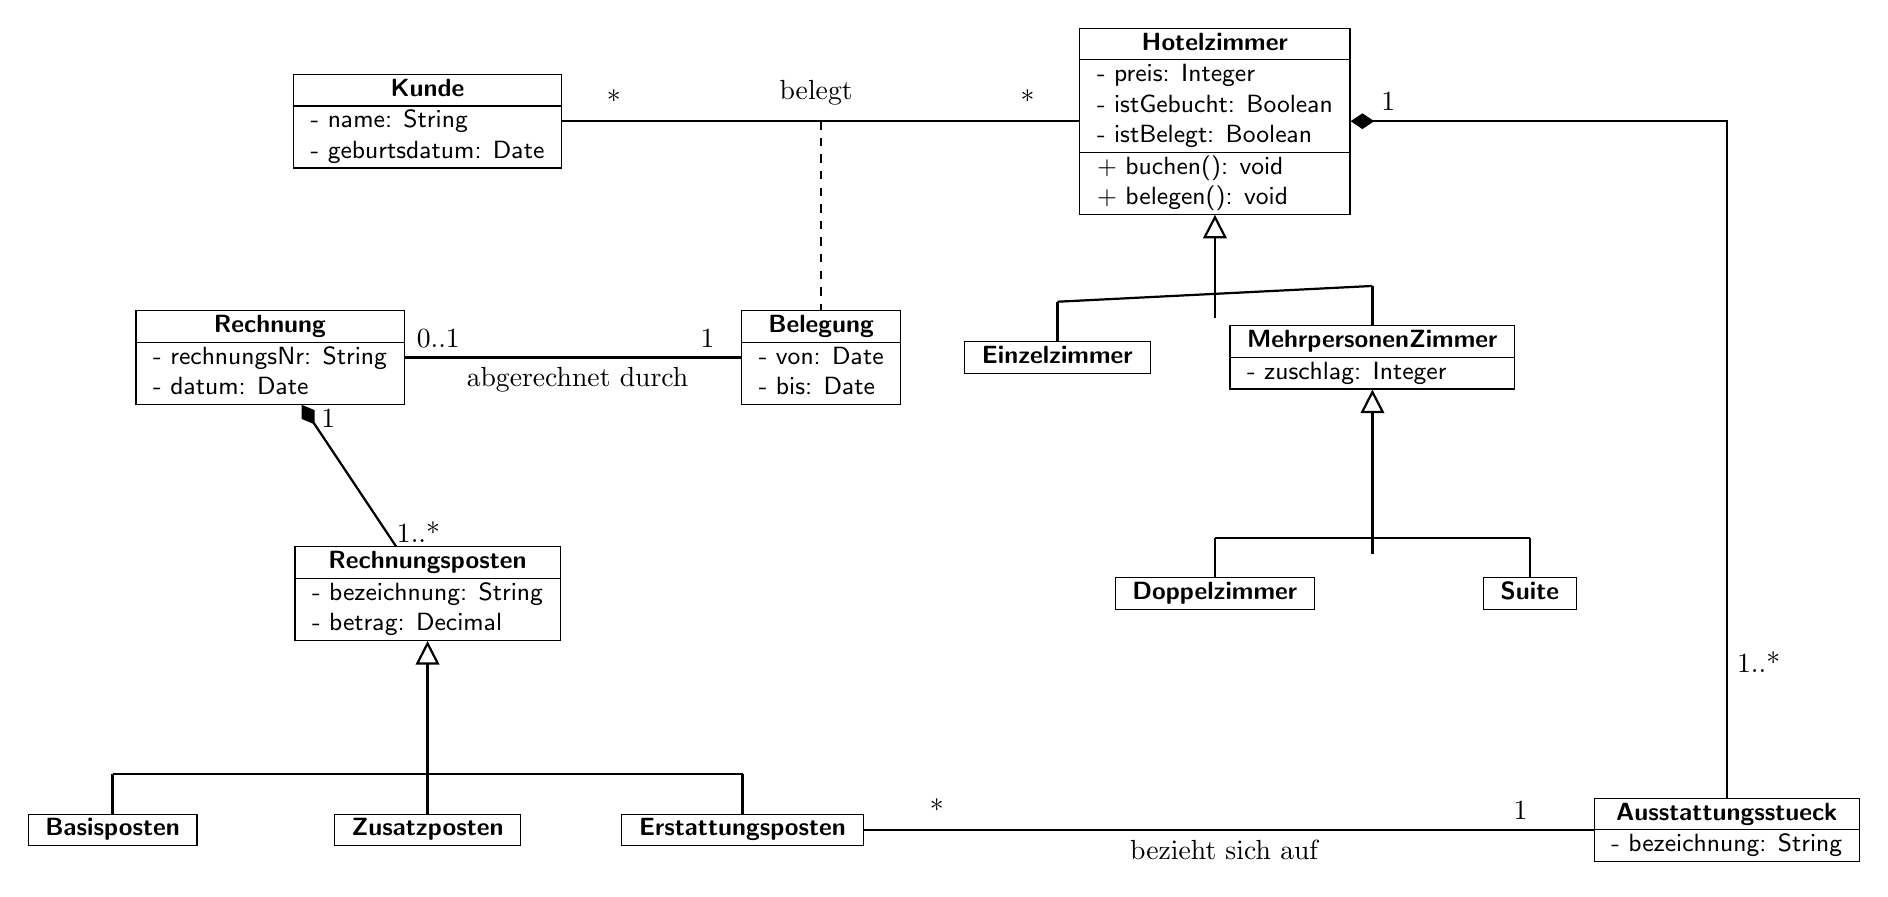
\begin{tikzpicture}[
            % ----- Styles -----
                class/.style={
                    inner sep=0pt,
                    outer sep=0pt,
                    font=\small\sffamily
                },
                inher/.style={-{Triangle[open, length=3mm, width=3mm]}, thick},
                comp/.style={{Diamond[length=3mm, width=2mm]}-, thick},
                assoc/.style={thick}
            ]

% ===================== Klassen (Tabulars in Nodes) =====================

% --- Obere Reihe (y=5): Basis-Klassen der Hauptassoziation ---
                \node[class] (Kunde) at (0, 5) {
                    \begin{tabular}{|l|}
                        \hline
                        \multicolumn{1}{|c|}{\textbf{Kunde}} \\
                        \hline
                        - name: String \\
                        - geburtsdatum: Date \\
                        \hline
                    \end{tabular}
                };

                \node[class] (Hotelzimmer) at (10, 5) {
                    \begin{tabular}{|l|}
                        \hline
                        \multicolumn{1}{|c|}{\textit{\textbf{Hotelzimmer}}} \\
                        \hline
                        - preis: Integer \\
                        - istGebucht: Boolean \\
                        - istBelegt: Boolean \\
                        \hline
                        + buchen(): void \\
                        + belegen(): void \\
                        \hline
                    \end{tabular}
                };

% --- Mittlere Reihe (y=2): Assoziationsklasse & Rechnung ---
                \node[class] (Belegung) at (5, 2) {
                    \begin{tabular}{|l|}
                        \hline
                        \multicolumn{1}{|c|}{\textbf{Belegung}} \\
                        \hline
                        - von: Date \\
                        - bis: Date \\
                        \hline
                    \end{tabular}
                };

                \node[class] (Rechnung) at (-2, 2) {
                    \begin{tabular}{|l|}
                        \hline
                        \multicolumn{1}{|c|}{\textbf{Rechnung}} \\
                        \hline
                        - rechnungsNr: String \\
                        - datum: Date \\
                        \hline
                    \end{tabular}
                };

% --- Zimmer-Hierarchie (y=2 bis y=-1) ---
                \node[class] (Einzelzimmer) at (8, 2) {
                    \begin{tabular}{|l|}
                        \hline
                        \multicolumn{1}{|c|}{\textbf{Einzelzimmer}} \\
                        \hline
                    \end{tabular}
                };

                \node[class] (MehrpersonenZimmer) at (12, 2) {
                    \begin{tabular}{|l|}
                        \hline
                        \multicolumn{1}{|c|}{\textit{\textbf{MehrpersonenZimmer}}} \\
                        \hline
                        - zuschlag: Integer \\
                        \hline
                    \end{tabular}
                };

                \node[class] (Doppelzimmer) at (10, -1) {
                    \begin{tabular}{|l|}
                        \hline
                        \multicolumn{1}{|c|}{\textbf{Doppelzimmer}} \\
                        \hline
                    \end{tabular}
                };

                \node[class] (Suite) at (14, -1) {
                    \begin{tabular}{|l|}
                        \hline
                        \multicolumn{1}{|c|}{\textbf{Suite}} \\
                        \hline
                    \end{tabular}
                };

% --- Rechnungsposten-Hierarchie (y=-1 bis y=-4) ---
                \node[class] (Rechnungsposten) at (0, -1) {
                    \begin{tabular}{|l|}
                        \hline
                        \multicolumn{1}{|c|}{\textit{\textbf{Rechnungsposten}}} \\
                        \hline
                        - bezeichnung: String \\
                        - betrag: Decimal \\
                        \hline
                    \end{tabular}
                };

                \node[class] (Basisposten) at (-4, -4) {
                    \begin{tabular}{|l|}
                        \hline
                        \multicolumn{1}{|c|}{\textbf{Basisposten}} \\
                        \hline
                    \end{tabular}
                };

                \node[class] (Zusatzposten) at (0, -4) {
                    \begin{tabular}{|l|}
                        \hline
                        \multicolumn{1}{|c|}{\textbf{Zusatzposten}} \\
                        \hline
                    \end{tabular}
                };

                \node[class] (Erstattungsposten) at (4, -4) {
                    \begin{tabular}{|l|}
                        \hline
                        \multicolumn{1}{|c|}{\textbf{Erstattungsposten}} \\
                        \hline
                    \end{tabular}
                };

% --- Ausstattungsstück (unten rechts, y=-4) ---
                \node[class] (Ausstattungsstueck) at (16.5, -4) {
                    \begin{tabular}{|l|}
                        \hline
                        \multicolumn{1}{|c|}{\textbf{Ausstattungsstueck}} \\
                        \hline
                        - bezeichnung: String \\
                        \hline
                    \end{tabular}
                };


% ===================== Beziehungen & Assoziationen =====================

% Kunde --- Hotelzimmer (* --- *) mit Assoziationsklasse Belegung
                \draw[assoc] (Kunde) -- (Hotelzimmer)
                node[pos=0.1, above] {*}
                node[pos=0.9, above] {*}
                node[midway, above=2pt] {belegt $\blacktriangleright$};

% Verbindungslinie zur Assoziationsklasse Belegung
                \draw[dashed, thick] (5, 5) -- (Belegung.north);

% Belegung --- Rechnung (1 --- 0..1)
                \draw[assoc] (Belegung) -- (Rechnung)
                node[pos=0.1, above] {1}
                node[pos=0.9, above] {0..1}
                node[midway, below] {$\blacktriangleleft$ abgerechnet durch};

% Rechnung *--- Rechnungsposten (Composition: 1 --- 1..*)
                \draw[comp] (Rechnung) -- (Rechnungsposten)
                node[pos=0.1, right] {1}
                node[pos=0.9, right] {1..*};

% Erstattungsposten --- Ausstattungsstueck (* --- 1)
                \draw[assoc] (Erstattungsposten) -- (Ausstattungsstueck)
                node[pos=0.1, above] {*}
                node[pos=0.9, above] {1}
                node[midway, below] {bezieht sich auf $\blacktriangleright$};

% Hotelzimmer *--- Ausstattungsstueck (Composition: 1 --- 1..*)
                \draw[comp] (Hotelzimmer.east) -| (Ausstattungsstueck.north)
                node[pos=0.05, above] {1}
                node[pos=0.9, right] {1..*};


% ===================== Vererbungshierarchien =====================

% 1. Hotelzimmer -> Einzelzimmer, MehrpersonenZimmer
                \draw[thick] (Einzelzimmer.north) -- ++(0, 0.5) coordinate (h1);
                \draw[thick] (MehrpersonenZimmer.north) -- ++(0, 0.5) coordinate (h2);
                \draw[thick] (h1) -- (h2);
                \draw[inher] (10, 2.5) -- (Hotelzimmer.south);

% 2. MehrpersonenZimmer -> Doppelzimmer, Suite
                \draw[thick] (Doppelzimmer.north) -- ++(0, 0.5) coordinate (m1);
                \draw[thick] (Suite.north) -- ++(0, 0.5) coordinate (m2);
                \draw[thick] (m1) -- (m2);
                \draw[inher] (12, -0.5) -- (MehrpersonenZimmer.south);

% 3. Rechnungsposten -> Erstattungsposten, Basisposten, Zusatzposten
                \draw[thick] (Basisposten.north) -- ++(0, 0.5) coordinate (r1);
                \draw[thick] (Erstattungsposten.north) -- ++(0, 0.5) coordinate (r3);
                \draw[thick] (r1) -- (r3);
                \draw[inher] (Zusatzposten.north) -- (Rechnungsposten.south);

            \end{tikzpicture}
            \caption{UML Klassendiagramm -- Hotelverwaltungssystem}
            \label{fig:classdiagram}
        \end{figure}
    \end{landscape}

    \newpage

    %TODO: Aufgabe 8.3: UML Sequenzdiagramm
    \exercise{Abgabe 8.3: UML Sequenzdiagramm}

\end{document}
